\chapter{Motion Tracking}
Just to introduce the topic, we can say that motion tracking is the process of determining the movement of an object in a video sequence. 
More in general, it regards the understanding of \textit{what} is moving in a scene and \textit{how} it moves or interacts with the environment.

This is a very important topic in computer vision, and it is used in many applications, such as video surveillance, traffic monitoring, human-computer interaction and biological applications (such as cell tracking). 
At high level, motion tracking can be used for the discovery of activities, behavior understanding, and detection of threats.

In this chapter, we will discuss the basic concepts of motion tracking, and we will present some of the most common algorithms used in this field.

\section{Object Tracking}
Object tracking is the process of continuously locating a moving object over time. 
Depending on the application's requirements, tracking can be done in various ways: tracking the 2D coordinates of an object's centroid, tracking in 3D (which requires multiple cameras), or determining the positions of complex objects, such as the articulations of a human body.

The primary goal of object tracking is to estimate the object's state in each frame and predict its future position. 
This capability has a wide range of applications. In monitoring and surveillance, object tracking can be used for motion classification, identifying anomalous or suspicious behaviors, and following a trajectory.

In human-machine interfaces, it enables interaction with devices without physical barriers like a mouse or keyboard, and aids in natural language understanding. 
In virtual reality, object tracking contributes to creating immersive experiences and animating virtual characters.

Additionally, object tracking is valuable in mining and retrieval applications, such as browsing databases for specific motion patterns. 
Overall, object tracking is a versatile technology with numerous practical uses across various fields.
\\
Some benefits of object tracking are:
\begin{itemize}
\item In HCI, control PC (or systems in general) $\Rightarrow$ no need for additional tools;
\item In surveillance, Automated / Semi-automated systems $\Rightarrow$ reduce the stress of human operators;
\item Virtual reality, computer animation $\Rightarrow$ animate and drive the avatar;
\item But also: Training of athletes, Gait disorders detection, Medical applications, etc.
\end{itemize}

\section{2D Tracking}
Sometimes it is enough to track the object in 2D, for example when the object is moving on a plane.
Exists different approaches to 2D tracking:
\begin{itemize}
\item \textbf{Region-based} $\Rightarrow$ set of pixels that share similar features (color). This does not work very well with multiple objects moving at the same times, on top of that it's computationally intensive;
\item \textbf{Contour-based} $\Rightarrow$ determine position and shape of an object over time. Useful to track deformable objects;
\item \textbf{Feature-based} $\Rightarrow$ select meaningful points (contours, corners). Very common and effective method, relevant points are selected and tracked over time;
\item \textbf{Template-based} $\Rightarrow$ use specific models (hands, faces, eyes).
\end{itemize}

\subsection{Region-based tracking}
When it comes to real-time applications, tracking regions with uniform appearance offers several benefits. 
It enables swift processing, often exceeding 30 frames per second, while maintaining a commendable balance between quality and speed. 
The idea revolves around identifying areas in an image that exhibit consistent color characteristics. 
These regions are akin to patches of similar color projected onto the image plane, often achieved through segmentation techniques like background suppression.

One fundamental requirement for successful region tracking is ensuring that these regions possess distinguishable colors. 
However, this method faces challenges, particularly in scenarios with variable illumination. 
Changes in lighting conditions can destabilize the uniformity of color, complicating the tracking process. 
To mitigate this issue, various compensation techniques can be employed, such as utilizing the hue and saturation components of the HSV color space or normalizing the RGB values. 
While these techniques work reasonably well indoors, outdoor settings may present more difficulties due to unpredictable lighting changes.

In terms of what we aim to track, the possibilities are diverse. 
It could involve monitoring any moving object, distinguishing between skin and non-skin regions (useful for applications like hand and face tracking), identifying specific colored areas, and more. 
The approach typically involves techniques such as color thresholding for uniform regions or utilizing color histograms. 

However, tracking regions with uniform appearance isn't without its challenges. 
Color variations over time due to changes in illumination or object posture pose significant hurdles. 
Additionally, models of tracked objects need continual updates to adapt to evolving conditions.

One conceivable approach to tackle these challenges involves breaking down the object into smaller regions. 
Each region is then associated with a \textit{color vector} or histogram, representing the average color values within that region. 
During tracking, the color of each region is computed, and the similarity to a reference model is assessed. 
If the ratio between the reference and current values is close to 1, it indicates a good match.

Histograms serve as a valuable tool in this process. 
They provide a quantified representation of the color distribution within a region, enabling comparisons between reference and current models. 
\\Different similarity measures can be employed for evaluation, such as bin-by-bin comparison: 
\[
    \bigcap (O_i^t, O_i^r) = \sum_{n=1}^{U} min \{O_{i,n}^r, O_{i,n}^t\} 
\]

\begin{figure}[H]
    \centering
    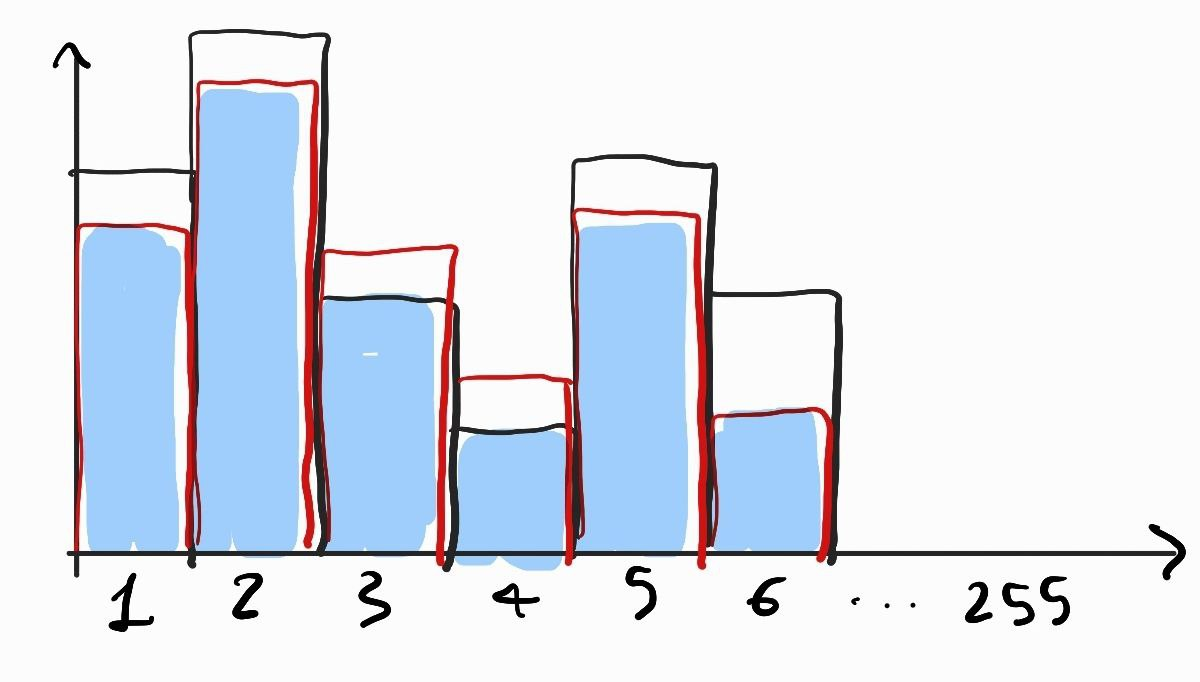
\includegraphics[width=0.4\textwidth]{Figures/bins.jpg}
    \caption{For all the bins of each object we compute the \\intersection (blue), one that
    yields the highest value is the best match.}
    \label{fig:bins}
\end{figure}

or Sum of Squared Differences (SSD), so instead of computing the correlation between the two histograms, we compute the difference between the two histograms, the error: 
\[ 
    SSD(O_i^t, O_i^r) = \sum_{n=1}^{U} (O_{i,n}^r - O_{i,n}^t)^2 
\]
Careful consideration must be given to the number of bins used in the histograms, striking a balance between granularity and computational efficiency. A smaller number of bins may also lead to better generalization, as it reduces the impact of noise.

In summary, tracking regions with uniform appearance offers a promising avenue for real-time applications, but it requires robust techniques to address challenges such as variable illumination and color changes over time. 
Techniques involving region division and histogram analysis can help achieve accurate and efficient tracking in these scenarios.
\\\textit{NB: Shadows can be problematic in region-based tracking as they introduce noise, leading to false positives. 
A shadow does not correspond directly to the motion of a real object; rather, if we are lucky enough, it represents a change in the object's color, specifically a variation in luminance while chrominance remains ideally unaltered. 
To ensure proper tracking, shadows should be removed beforehand using a suitable algorithm.}

\section{Blobs extraction} 
An object can consist of multiple blobs, such as one for the torso and one for the head, disjoint one from the other. Blobs are aggregations of connected pixels that share common features. 
When considering features, position is also important, so pixels with similar color but located far from the object must be discarded. 
This approach is typically used in combination with background suppression to enhance object detection and tracking.
\subsection{Target association}
This is a procedure common to all trackers, not only region-based. In general, it is worth noting that detection is not carried out on a frame-basis.
This could lead to a lot of false positives, and it is computationally expensive.  
The idea is that once detected, targets are followed on a proximity basis. 
So, for example, background subtraction informs about the presence of motion, histograms characterize each moving objects, and then, unless occlusion occur, the target in the next frame should be the closest blob.
\begin{figure}[h]
\centering
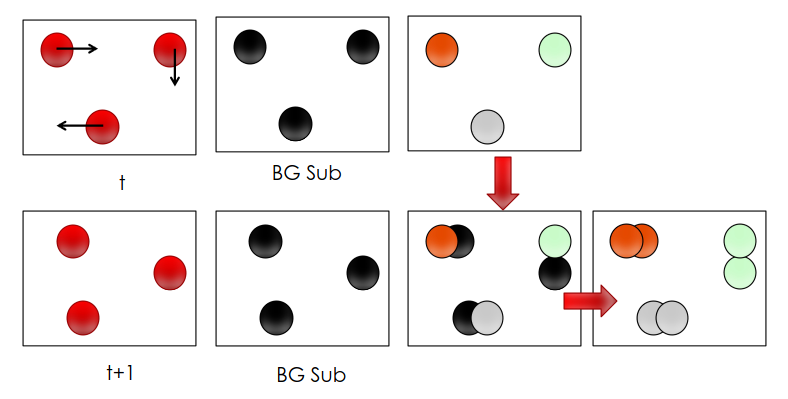
\includegraphics[width=0.7\textwidth]{Figures/Target_association.png}
\end{figure}

The steps of target association can be summed up as follows:
\begin{itemize}
\item Overlapping blob (issues with scale $\Rightarrow$ depends on objects size);
\item Centroid with minimum distance (as above);
\item Overlapping bounding boxes (may fail due to perspective);
\item Bounding box with minimum distance;
\item Bounding box to centroid distance.
\end{itemize}

\textit{NB: When association has been completed, for each object or blob update the appearance model to account for small variations. In presence of occlusions, the last saved model can be used to disambiguate.}

\subsection{Splitting}
Splitting is a common problem in blob extraction because an object can be made up of several blobs. 
If each object is identified as a single blob, there are no issues. 
However, background subtraction can give confusing results. 
Objects might be broken into several small blobs, meaning there isn't a clear separation between background and foreground. 
Similarly, two objects might enter the scene together and then separate.
\begin{figure}[h]
    \centering
    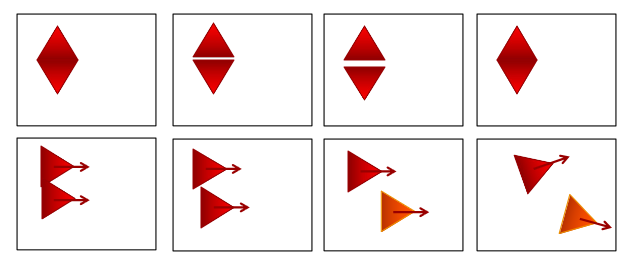
\includegraphics[width=0.7\textwidth]{Figures/Splitting.png}
\end{figure}\\
To figure out what's happening, it's important to gather more information over time. 
It's impossible to understand right away whether it's a single object that looks fragmented or two objects close together. 
Therefore, we need to observe for a while to decide if the blobs belong to one object or two separate ones.
\section{Merging}
\begin{wrapfigure}{r}{0.4\textwidth}
    \centering
    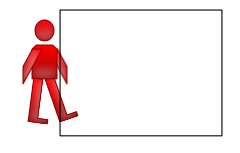
\includegraphics[width=0.25\textwidth]{Figures/Merging.png}
\end{wrapfigure}
Merging is the opposite of splitting, and it is due to the fact that two objects are identified as a single blob. This can happen when two objects are close to each other and move together consistently (then perhaps they're the same object).
An example can be when a person’s arm and foot enter the scene first and are detected as two well-separated FG blobs. 
Then also the rest of the body enters, and a single blob is created. 

\subsection{Criteria for splitting and merging}
Observation is crucial in determining whether regions should be split or merged. 
To make accurate decisions, we need to monitor regions of interest and evaluate their consistency based on several factors. 
Consistent direction of motion can indicate that multiple regions belong to the same object, while the distance between centroids or bounding boxes helps to identify whether regions are part of the same object based on their proximity. 
By observing the temporal range, we can determine if regions consistently behave as a single entity over time. 
Additionally, regions moving at similar speeds are likely part of the same object, and feature matching (comparing characteristics like color, texture, or shape) further aids in deciding whether regions should be considered as one object. 
Evaluating these criteria ensures more accurate tracking and identification of objects.

\section{Occlusion}
Occlusion is an anomalous, but very frequent, situation in tracking, and it occurs when moving objects overlap.
Consequently, one or more objects disappear from the scene and bigger blobs appear as a result of the occlusion, with properties that don't belong to any of the models acquired previously, so the acquisition models are not reliable anymore.
\\\textit{NB: Model update should be avoided during occlusions.}

In order to solve this problem, we need to re-associate "A to A" and "B to B" (where A and B are the objects that are occluded). 
\\\textit{NB: Histograms are a good way out.}

\section{Tracking: Feature-based}

Histograms are just one way to track objects, we also mentioned other methodologies, such as feature-based tracking. The objective is to retrieve the motion information from sets of features (such as points, corners, edges\dots) in local areas of the image.
\\Considering a set of images
\[
    A = \{A(0), A(1), A(2), \dots, A(j-1)\}
\] 
and the position of the feature in the image plane in each frame:
\[
    m_i(x_i, y_i)\;\;i = [0, j-1] 
\] 
\begin{wrapfigure}{r}{0.2\textwidth}
    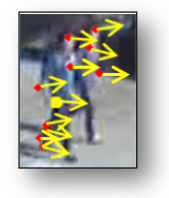
\includegraphics[scale=0.3]{Figures/Tracking.png}
\end{wrapfigure}
The objective is to determine the displacement vector:
\[
    d_i = (dx_i, dy_i)
\] 
That best estimates the position of the feature in the next frame:
\[
    m_{i+1}(x_{i+1}, y_{i+1}) = m_i + d_i
\]

We'd like to get the coordinated \(x\) and \(y\) of the feature in the next frames at time \(i+1\).
(In principle a feature point does not convey much information, usually we group them to create a bounding box or a convex hull that can contain the moving object into an independent structure).

The question now is how to choose a good feature point. Generally speaking it should have distinctive characteristics such as brightness, contrast, texture, edges, corners or points with high curvature, basically something that exhibits some elements that let that point be sufficiently diverse compared to the rest of the image.

We can use the \textbf{Good Features to Track} algorithm:
\[
    Z = \begin{bmatrix}
        \sum_{W}^{}J_x^2 & \sum_{W}^{}J_xJ_y \\
        \\
        \sum_{W}^{}J_yJ_x & \sum_{W}^{}J_y^2
    \end{bmatrix}
\]
\\Where $J_x$ and $J_y$ are the gradients evaluated on a certain point in the $x$ and $y$ direction within a certain window $W$ (of size $n\times n$). 
A good feature point is the with strong gradients component in both directions, so we are interested not only in the \(x\) and \(y\) components but also in the cross-correlation between them. To maximize this function we compute the eigenvalues of the matrix. In order to evaluate if it's a good feature point we are interested whether the smallest eigenvalue is larger than a certain threshold. This means that in case we have just one of the eigenvalues with high magnitude and the other very small probably it is a feature point with good characteristics only in one direction, what we are looking for is a point with strong components in \textit{both} directions, in practice, it highlights corner points and texture.

In summary, it's important to consider the following key points when analyzing eigenvalues:
\begin{itemize}
    \item Eigenvalues should surpass the image noise level to ensure reliable information.
    \item Small eigenvalues indicate strong similarity within the analyzed window.
    \item Presence of one large and one small eigenvalue suggests unidirectional patterns in the image.
    \item Points with two large eigenvalues are of high interest, indicating features like salt and pepper texture or corners.
\end{itemize}

For what concerns tracking, we must ensure that the same points are tracked throughout the video sequence. 
Ideally we would expect that $A_i(Dm-d)=A_{i+1}(m)$, where $A_i, A_{i+1}$ are the successive frames at time $i$ and $i+1$, $m$ is the 2D position of the feature point, $D$ the deformation matrix (affine transformation model) and $d$ is the displacement vector (translation models).
\\ However, due to noise the equality usually does not hold. In addition, since motion across successive frames is assumed to be small, a \textit{translational model} is a good approximation and the term $D$ can be removed. So, after making this simplification, we can use it to find the configuration of the displacement vector $d$ that \textit{minimizes} the residual between the two frames:
\[
    \varepsilon = \iint_{W} \left[A_i(m-d)-A_{i+1}(m)\right]^2 \omega(m) \, dm
\]
we are also implementing a weighting function $\omega$ such as Gaussian to emphasize the center of the window giving less relevance to the terms that are outside the center.

Inside the scene we are observing a lot of things can happen, for example the points we are looking for get occluded, exit the scene, or change color. In that situation the dissimilarity grows a lot. When the feature dissimilarity grows too large, the feature point should be abandoned and a new one should be selected.
To minimize the residual we differentiate and zero w.r.t unknowns ($d$)
\[
    e = 2 \iint_{W} \left[A_i(m)-A_{i+1}(m)\right]g(m) \, \omega(m) \, dm
\] 
and 
\[
    g(m)=\begin{bmatrix}
        \frac{\partial (A_i(m)-A_{i+1}(m))}{\partial x} \\
        \\
        \frac{\partial (A_i(m)-A_{i+1}(m))}{\partial y} 
    \end{bmatrix}
\]
In this case the solution for the displacement vector can be expressed by the 2x2 linear system of equations (see paper for details):

\[
    Zd = e
\]

The typical combination and feature detection and feature tracking takes as input the \textit{Good features to track} algorithm for the detection which is coupled to another algorithm for the tracking, such as the Lucas-Kanade optical flow.

\subsection{The Lucas-Kanade optical flow}
Substantially is a two-frame differential method for optical flow estimation.
Consider $u=[u_x, u_y]$ in frame $I$ and $v=[v_x, v_y]$ in frame $J$ the goal is to find $d$ that satisfies the equation $v = u + d$ such as $I$ and $J$ are similar(translation model).
We are not expecting rotations or distortions, for this reason the similarity is defined in the 2D domain.
$d$ is the vector that minimizes
\[
    \epsilon(d) = \epsilon(d_x, d_y) = \sum_{x=u_x-w_x}^{u_x+w_x} \sum_{y=u_y-w_y}^{u_y+w_y} \left[I(x, y) - J(x+d_x, y+d_y)\right]^2
\]

This above is pretty much the same thing we have seen before substituting the continuous integral with a discrete summation. The $\omega$ function has now become a window of size $w_x \times w_y$ centered in $u_x, u_y$.

\subsection{Pyramidal implementation}

The strong point of the Lukas-Kanade optical flow is the pyramidal implementation. In order to be a good tracker we need to satisfy two requirements: accuracy and robustness.

\textit{Accuracy} relates to the local sub-pixel accuracy attached to tracking, we want smoothness and to preserve detail information $\Rightarrow$ \textbf{small} integration window preferable

\textit{Robustness} relates to the sensitivity of tracking with respect to changes of light and big motions. We never know what's going to happen in the scene $\Rightarrow$ \textbf{large} integration window preferable

\begin{figure}[H]
    \centering
    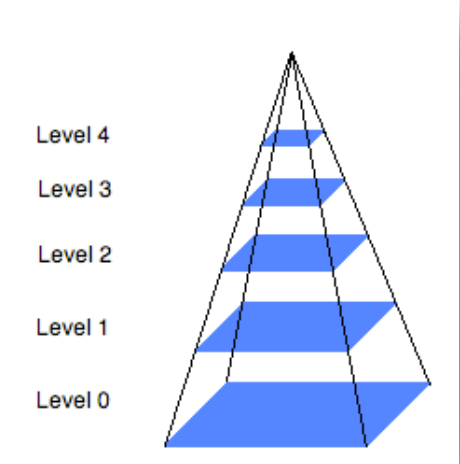
\includegraphics[width=0.2\textwidth]{Figures/pyramid.png}
    \caption{Pyramidal representation of the Lukas-Kanade optical flow.}
    \label{img:pyramid}
\end{figure}

In order to satisfy both requirements, the authors built a tracker which works on multiple scales. It means we are not working on a single image, instead we are working on a number of levels, small movements in the higher levels correspond to big movements in the lower levels, as shown in Figure \ref{img:pyramid}.

\begin{itemize}
    \item Level 0 is the image at original resolution.
    \item Level 4 is the image at lowest resolution.
    \item The L-th level is defined as a linear combination of the elements in the previous level.
\end{itemize}
\(
    I^L(x,y) = 
\)\\
\(
    \frac{1}{4}I^{L-1}(2x, 2y)+
\)\\
\(
    \frac{1}{8}(I^{L-1}(2x-1,2y) + I^{L-1}(2x+1,2y)+I^{L-1}(2x,2y-1)+I^{L-1}(2x,2y+1))+    
\)\\
\(
    \frac{1}{16}(I^{L-1}(2x-1,2y-1) + I^{L-1}(2x+1,2y+1)+I^{L-1}(2x-1,2y+1)+I^{L-1}(2x+1,2y-1))    
\)

To construct higher levels, the contributions of the pixels around the pixel in the lower level are taken into account and weighted. Then what we do is that we start our analysis from the highest level, the smallest. How do we do that?

\[
\epsilon^L(d^L) = \epsilon^L(d^L_x, d^L_y) = \sum_{x=u^L_x-w_x}^{u^L_x+w_x} \sum_{y=u^L_y-w_y}^{u^L_y+w_y} \left[I^L(x, y) - J^L(x+ g^L_x +d^L_x, y+g^L_y+d^L_y)\right]^2
\]

Starting from the lowest level we make a guess of the flow \textbf{g} and, looking at the observation window, we find the first displacement vector, this means that after minimizing the quantity $\epsilon$ we have an initial guess of the displacement.
\\

After that we go to the lower, bigger level. Scaling the motion vector as it doubles its scale, but now we have more pixels and a better chance or refining the guess just by looking in the new neighborhood and fine-tuning the displacement vector. The propagation of information to the lower levels follows this equation:

\[
    g^{L-1} = 2(g^L+d^L)
\]

Overall the displacement becomes:

\[
    d = \sum_{L=0}^{L_{max}} 2^Ld^L    
\]



\subsection{Bayesian tracking}

The approaches seen so far were based on the assumption we were computing some sort of distance that would give us the chance to find again the point of interest within a certain neighborhood, we will now see an extension of this approach, by giving it a probabilistic twist.

We are considering the tracking problem as a process in which we are making \textbf{estimations} about the position of the object given a certain evidence that we are collecting over time. We represent the state of a system in terms of $x$ and $y$ coordinates but not only, we also take into account the \textit{velocity} and the \textit{acceleration} of the object along both dimension.

The point in this image plane will have a 6D state vector that will describe the state of our system at a given time instant. We expect and take into account noise, but we assume that it's smaller than the amount of information about the state.

\[
    x_k = f_k(x_{k-1}, w_{k-1})
\]

The state $x$ at time $k$ can be seen as a function that depends on the previous state of the system plus some noise $w$ that we need to consider making a proper analysis. The process noise is whatever cannot be controlled directly and \textit{just happens}.

\[
    z_k = h_k x_k + v_k
\]

In order to make the prediction it's not enough to just rely on the initial position of the subject and just propagate this information about the speed, because there's noise. In Bayesian Tracking when necessary we take a \textit{measurement} trying to confirm our hypothesis. Our measurement $z_k$ is the result of a funtion $h_k$ which takes into account the state of the system plus some measurement noise $v_k$ (may be due to discrete pixels, ambiguous shape etc...).
\\
\\
We can now construct a model in a way that we can start from a prediction, take a measurement "on the ground" and, similarly to Lukas-Kanade, check if the measurement is in line with the prediction, if not we can correct the measurement, the correction that we take (the measurement of the displacement between prediction and measurement) will guide us in the next step.
\\
\\
We are working \textit{online}, using an observation to perform an estimate. More formally we can say that the initial PDF of the state of the system should be given, we should know \textit{at least} the objects that we are going to track, once we know what we are looking for we can take as initial starting point the initial probability $p(x_0|z_0)$ where at the beginning $z_0$ contains no measurements. Our goal is,  for every time step $k$, to compute $p(x_k|z_k)$, the probability of the state of the system given the measurements we have taken up to that time instant.


We have said that:
\[
    x_k = f_k(x_{k-1}, w_{k-1}) \rightarrow p(x_k|x_{k-1})
\]
\[
    z_k = h_k(x_k, v_k) \rightarrow p(z_k|x_k)
\]

Considering these two quantities we can create a model for the estimation of the state of the system that consists of these formulations:

\[
    p(x_k|z_{k-1}) = \int p(x_k|x_{k-1})p(x_{k-1}|z_{k-1})dx_{k-1}
\]

\begin{multicols}{3}
    Prior at time step k\\
    System model\\
    Posterior pdf at k-1
\end{multicols}

We want to create a prior $p(x_k|z_{k-1})$ meaning that I have taken a measurement in the previous step, this measurement relates to that state of the system $k-1$, and thanks to this measurement I can create a \textit{prior}, I can project this measurement ahead in time to give me the new state $x_k$.

And how is this computed? I can use some posterior information, which is the correction of our $k-1$ prediction given the measurement, this corrected piece of information is propagated forward through our \textbf{system model} $p(x_k|x_{k-1})$ which tells me how to go from $x_{k-1}$ to $x_k$. 

Using the Bayes theorem it is possible to obtain the desired pdf:

\[
    p(x_k|z_k) = \frac{p(z_k|x_k)p(x_k|z_{k-1})}{p(z_k|z_{k-1})}
\]

Where $p(z_k|z_{k-1})$ is used for normalization and computed as

\[
    p(z_k|z_{k-1}) = \int p(z_k|x_k)p(x_k|z_{k-1})dx_k
\]

\begin{figure}[H]
    \centering
    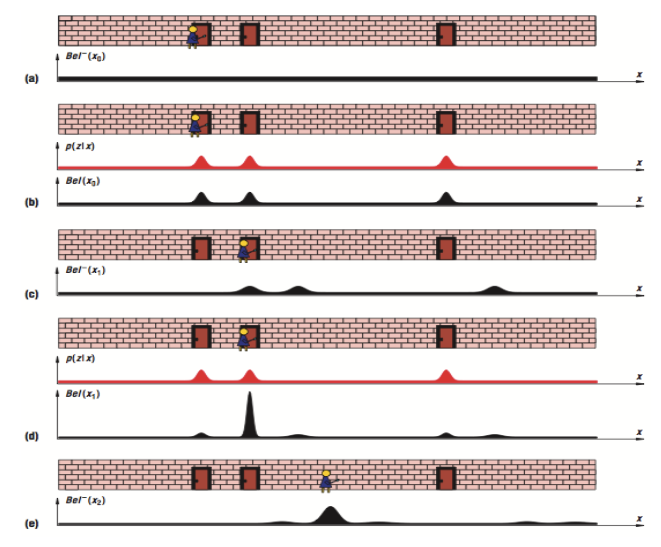
\includegraphics[width=0.95\textwidth]{Figures/bayes.png}
    \caption{Bayesian tracking toy example.}
    \label{img:bayes}
\end{figure}

In the toy example \ref{img:bayes} the person is equipped with a "door sensing device" and we assume constant speed. 


\begin{description}

\item [(a)] We can see how at the very beginning we have no idea where the person is, so our estimation about the position of the person is that it's anywhere in the area.
\item [(b)] What happens next is that the guy approaches a door we get a signal, but we only have that information, the person could be at any of the three positions, so our $p(z|x)$, the probability of a measurement given a state of the system, raises 3 peaks in correspondence of the three possible positions of the person, the doors. This becomes out a posteriori information which is something that we are storing and we need to propagate ahead  in time.
\item [(c)] We can propagate the a posteriori information ahead in time using the system model, in this case, the constant speed model, and we can see that the peaks are moving to the right, this is the prediction of the system. We also know that the uncertainty is increasing, this is due to the noise, for this reason the peaks are getting wider.
\item [(d)] At this point the door sensing device starts ringing again, meaning the guy has reached one of the other 3 doors. We don't know which one but given our model propagated in time, we can construct a new a posteriori taking into account $Bel^{-}(x_1)$ and the new measurement $p(z|x)$ and, while we still have some components due to noise, we are quite sure that the guy is at the second door.
\item [(e)] As we progress over time, we propagate the information, the uncertainty increases until at some point we get a new measurement.
\end{description}

\subsection{The Kalman Filter}

The idea of the Kalman filter goes back to Bayesian tracking. We take a prediction, validate that prediction with a measurement and knowing that both prediction and measurement are subject to noise, we can combine them in a way so that we can minimize the error in the estimation of the state of the system.
\\\\
We start from
\[
    z_1, \sigma^2_{z_1}    
\]
\[
    \hat{x}_1 = z_1
\]
\[
    \sigma^2_1 = \sigma^2_{z_1}    
\]

Where $z_1$ is the measurement that already includes some noise that we define with a variance $\sigma^2_{z_1}$. We provide the first prediction by initiating it at the first measurement location, and we just map the variance of the measurement to the variance of the prediction.

Starting from this we can propagate the information over time, make a new prediction, take a measurement, correct the measurement and make the new prediction and so on.
\[
    z_2, \sigma^2_{z_2}\;\;\;\;\hat{x}_2=?\;\;\;\;\sigma^2_2=?    
\]

We need to come up with a second measurement $z_2$ with its variance, make a new prediction and come up with a new value for the noise.

\begin{figure}[H]    
\[
    \hat{x}_2 = \hat{x}_1 + K_2(z_2-\hat{x}_1) \;\;\;\;\;\; K_2 = \frac{\sigma^2_1}{\sigma^2_1+\sigma^2_{z_2}}  
\]
\[
    \frac{1}{\sigma^2_2} = \frac{1}{\sigma^2_{z_1}}+\frac{1}{\sigma^2_{z_2}}\;\;\;\;\;
    \sigma^2_2 = \frac{\sigma^2_{z_1}\sigma^2_{z_2}}{\sigma^2_{z_1}+\sigma^2_{z_2}} 
\]
\caption{Simplified Kalman Filter.}
\label{eq:kalman}
\end{figure}
In the first equation we rely on the information we collected before, and we add a displacement to this quantity to get the new prediction $\hat{x}_2$ by taking into account some additional parameters. Capital K is what we call the \textbf{Kalman gain}, it's a multiplying factor which weights the distance between the second measurement $z_2$ and the previous estimate $\hat{x}_1$: we know that from the previous estimate and the new measurement we have an error, and so we use this error information together with the Kalman gain to push ahead our estimation. The Kalman Gain is a combination of the variances we are collecting. It's basically a weighted average between the prediction and the measurement, the weight is given by the ratio of the variances. 
\\

The process is rather simple because we basically have to iterate between these two steps, the first one is prediction and the second one is measurement: first we predict the new state and the correspondent uncertainty $\sigma^2$, then we correct using the new measurement $z$ for which we know there's a variance associated $\sigma^2_z$, this piece of information is the one that will guide us torwards the next prediction and variance.
\\

The Kalman Filter is also a computationally efficient solution to the least squares method. With LSM, we are trying to minimize an error, similarly with Kalman's formulation what we are trying to do is to find the configuration of the Kalman Gain (which is also the only parameter we can tune) to make sure that the result obtained from the prediction is as close as possible to the real position of the object.
\\

Assuming that the noise components $w_k$ and $v_k$ are normal distributions, the overall state and measurement model can be expressed through the following equations:

\[
    x_k = A_kX_{k-1}+B_kU_k+w_{k-1}    
\]
\[
    z_k = H_kx_k+v_k   
\]

Looking at the measurement equation we can see that the measurement is something that is going to happen on the basis of $x_k$ (we previously mentioned how $z_k$ is a function of $x_k$ and the noise) and this function is nothing but a multiplication of the measurement matrix $H_k$ and $x_k$, plus the noise contribution $v_k$.

Similarly, for the state information $x_k$ we have the system model $A_k$ which projects the state of the system at time $k-1$ forward in time. In this formulation we have an additional term $B_kU_k$ which is the control input: we can model additional information that we can inject into the system to guide the state of the system in a certain direction, for instance if we directly press gas on a car or if we adjust the trajectory of a missile.
\\

The noise in the process is usually modeled as a Gaussian distribution with zero mean and covariance matrix $Q$ and $R$:

\[
    p(w) = N(0, Q)
\]
\[
    p(v) = N(0, R)
\]

The error is one of the driving forces in our model, a very relevant parameter, in fact we have seen in Equation \ref{eq:kalman} how, if there's no noise, the Kalman Gain would disappear. Not only that, if the measurement is correct and the error zero we wouldn't be able to project ahead in time the state of the system.

\subsection{Predict-and-correct stages}

During the first phase the current state estimate together with the error estimate are propagated forward in time, in the second stage a new measurement is taken to modify the two estimations.
This gives us the chance to have an \textbf{a priori estimate} of the state of the system, before taking any new measurement, based only on the past knowledge; and an \textbf{a posteriori estimate} which is the corrected version of the a priori estimate, after taking the new measurement into account.
\\

\textit{NB: while maybe only Equation \ref{eq:kalman} is worth remembering by heart, we will quickly go through all of them to complete the pipeline}
\begin{figure}[H]
    \centering
    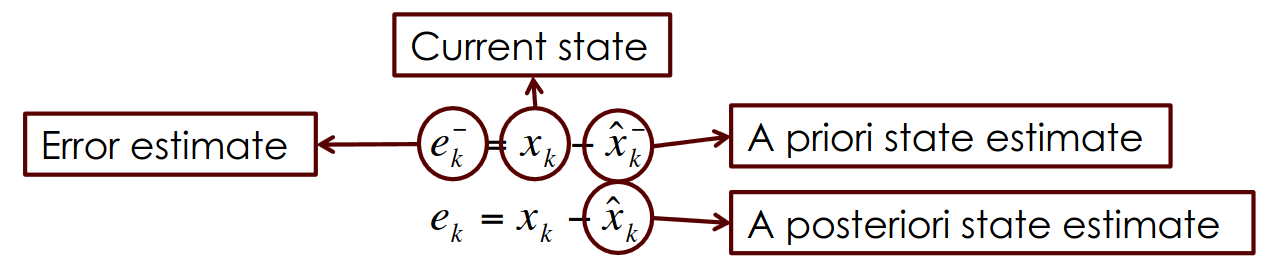
\includegraphics[width=0.8\textwidth]{Figures/prior.png}
    \caption{The minus means that it is an a priori information, modeled via our current state and our a priori estimate. This error allows us to make an a posteriori estimate $\hat{x}_k$ that will be used to estimate the new error and so on.}
    \label{img:prior}
\end{figure}

Once we have the error we can compute the covariance matrices, both a priori and a posteriori:

\[
    P^-_k = E[e^-_ke^{-T}_k]
\]
\[
    P_k = E[e_ke^T_k]
\]

After that we can start the prediction (the new a priori estimate) and compute the new error matrix (we are discarding the additional control parameter $B$ for simplicity):

\[
    \hat{x}^-_k = A_k\hat{x}_{k-1}
\]
\[
    P^-_k = A_kP_{k-1}A^T_k+Q_{k-1}
\]

This leads to the definition of the new Kalman Gain, which needs to take into account the error estimate:

\[
    K_k = P^-_kH^T_k(H_kP^-_kH^T_k+R_k)^{-1}    
\]

The gain is used to modify the a priori estimate and to compute the a posteriori state estimate:

\[
    \hat{x}_k = \hat{x}^-_k+K_k(z_k-H_k\hat{x}^-_k)
\]

And to compute the a posteriori error covariance, which is then used to compute the new prior and so on:

\[
    P_k = (I-K_kH_k)P^-_k    
\]

\begin{figure}[H]
    \centering
    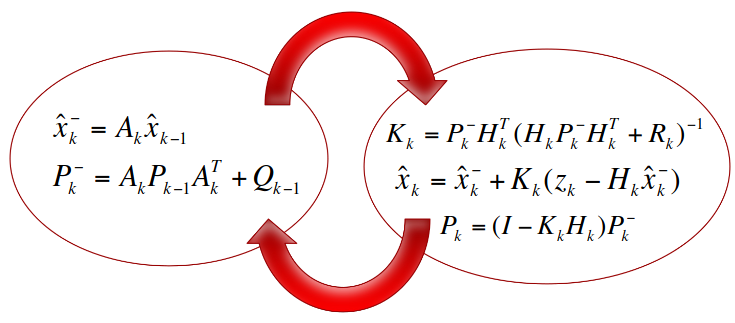
\includegraphics[width=0.8\textwidth]{Figures/loop.png}
    \caption{While \textit{it's not necessary to remember the equations} it must be clear how the information flows in the algorithm.}
    \label{img:loop}
\end{figure}

\subsection{Simple Kalman Filter example}

The situation is that we are trying to estimate the value of a constant function, the voltage out of a socket, we know that the voltage is 220V but we are not sure about the noise in both the measurement and in the process.

\begin{figure}[H]
    \centering
    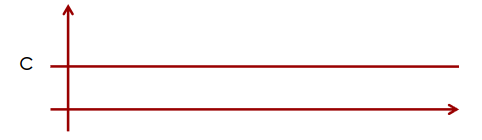
\includegraphics[width=0.7\textwidth]{Figures/constatn.png}
    \caption{The function we are trying to estimate.}
    \label{img:const}
\end{figure}

The problem is easy: obviously we know something about the model, otherwise it would be impossible to make an estimate, and knowing that this is a constant we are sure there's no evolution in both the model $A$ and the measurement $H$ matrices, so:

\[
  A = 1  
\]
\[
  H = 1  
\]
\[
  x_k= x_{k-1} + w_k
\]
\[
  z_k = x_k + v_k  
\]

Our a priori state estimate is given by the previous state and the error covariance is just changed by the presence of some noise:

\[
  \hat{x}^-_k = \hat{x}_{k-1}
\]
\[
    P^-_k = P_{k-1}+Q    
\]

At this point we just have to use the equation of the Kalman filter, compute the Kalman gain, thanks to that estimate the new posterior and the new error matrix:
\[
    K_k = P^-_k(P^-_k+R)^{-1}    
\]
\[
    \hat{x}_k = \hat{x}^-_k+K_k(z_k-\hat{x}^-_k)    
\]
\[
    P_k = (1-K_k)P^-_k    
\]

To make the algorithm work we just have to select as starting value the initial state "wrong" and the initial non-zero error covariance, then we can iterate the algorithm and see how the estimate converges to the real value of the function.

\begin{figure}[H]
    \centering
    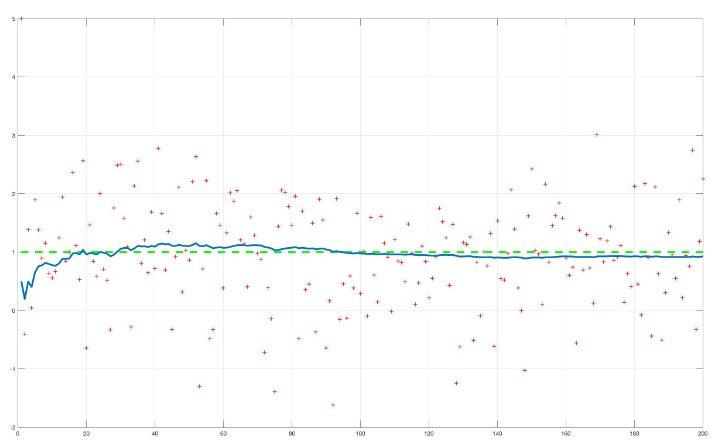
\includegraphics[width=0.7\textwidth]{Figures/voltage.png}
    \caption{The results of our simplified example.}
    \label{img:voltage}
\end{figure}

\subsection{Extended Kalman Filter}

An assumption that we made is that the behavior of the system is linear, the question is whether this reflects or not what happens in the real world. Turns out it does not.

The goal of the \textbf{Extended Kalman Filter (EKF)} is to adapt the Kalman Filter to linearize the equations that we used in the standard version. To define our state $x_k$ and measurement $z_k$ we are still using  $f_k$ and $h_k$, the only difference is that it's no more linear functions.

\[
  x_k = f_k(x_{k-1}, w_{k-1})  
\]
\[
    z_k = h_k(x_k, v_k)    
\]

Considering that we are assuming that the process is not linear, in order to linearize them we use partial derivatives of both $A$ and $H$. Since we don't know the values of noise we can assume here for simplicity that state and measurement are:

\[
    \tilde{x}_k = f(\hat{x}_{k-1},0)    
\]
\[
    \tilde{z}_k =  h(\tilde{x}_k,0)   
\]

Using the same notation as for KF, the \textbf{prediction} stage is given by:

\[
    \tilde{x}_k = f(\hat{x}_{k-1},0)    
\]
\[
    P^-_k = A_{k-1}P_{k-1}A^T_{k-1}+W_{k-1}Q_{k-1}W^T_{k-1}    
\]
\\
Where $A_k$ is the Jacobian matrix of partial derivatives of $f$ with respect to $x_k$.\\
$W_k$ is the Jacobian matrix of partial derivatives of $f$ with respect to $w_k$.\\
$Q_k$ is the process noise covariance matrix
\\
And the update loop becomes:

\[
    K_k = P^-_kH^T_k(H_kP^-_kH^T_k+V_kR_kV^T_k)^{-1}    
\]
\[
    \hat{x}_k = \tilde{x}_k+K_k(z_k-h_k(\tilde{x}_k,0))
\]
\[
    P_k=(I-K_kH_k)P^-_k    
\]
\\
$H_k$ is the Jacobian matrix of partial derivatives of $h$ with respect
to $x_k$
\\
$V_k$ is the Jacobian matrix of partial derivatives of $h$ with respect
to $z_k$
\\
$R_k$ is the measurement noise covariance matrix

\begin{figure}[H]
    \centering
    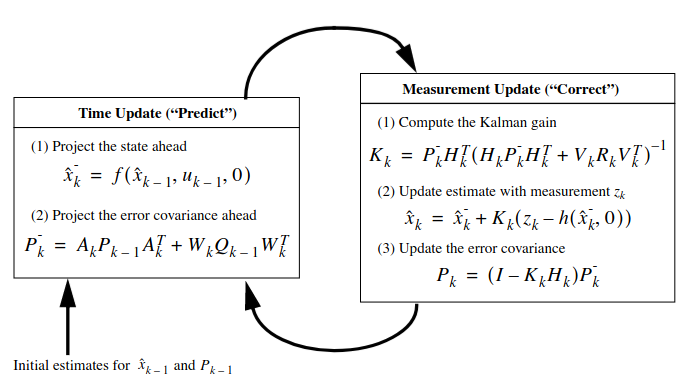
\includegraphics[width=0.7\textwidth]{Figures/update.png}
    \caption{This is the final update loop for the EKF.}
    \label{img:update}
\end{figure}

This helps us to deal with processes that are non-linear. However, this is only partially true in the sense that it's still very common to use the standard Kalman filter also in presence on non-linear processes with some approximations (the assumption that between two successive states we don't have big differences, so the non-linearity can be somewhat neglected), the EKF is used when the non-linearity is very strong.

\subsection{Particle Filters} 

Still, there are some situations where the EFK cannot provide satisfactory results. With \textbf{Particle Filters} the goal is to make it possible to track objects that are not only \textit{non-linear} but also that are behaving in a \textit{non-Gaussian} way.

The idea is to replace the single estimation that we are doing with KF and EFK with multiple representations: we are providing alternative solutions to our problem. 

\begin{figure}[H]
    \centering
    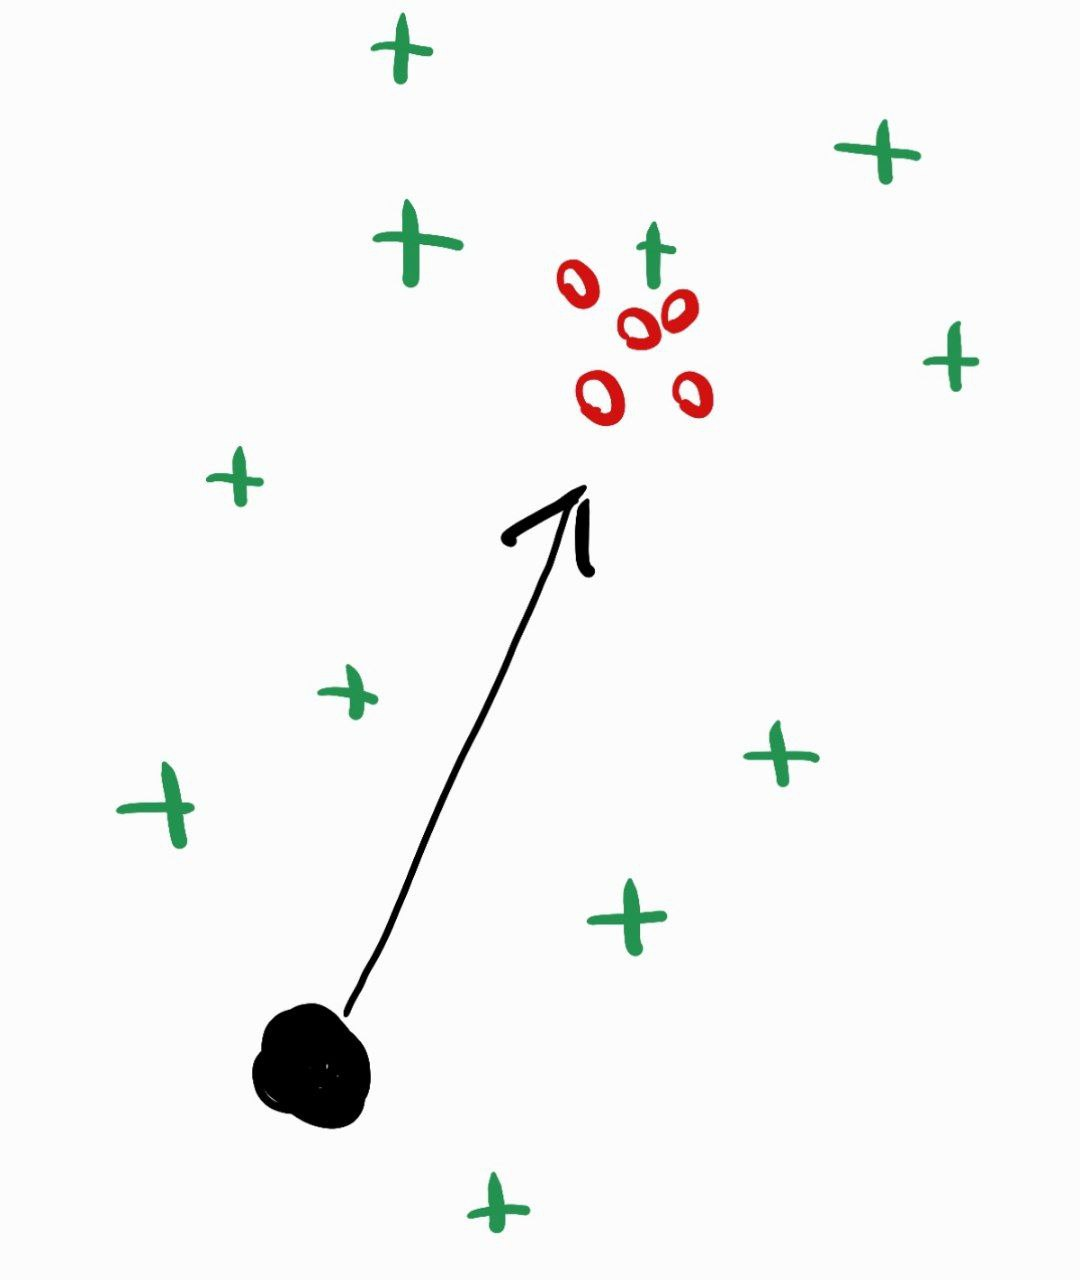
\includegraphics[width=0.25\textwidth]{Figures/nongaus.jpg}
    \caption{Red circles represent possible Gaussian predictions meanwhile the green crosses are possible predictions or hypothesis of a non-Gaussian model.}
    \label{img:nongaus}
\end{figure}

Instead of looking at a single point I'm checking multiple different solutions. The higher the number of particles the closer we are getting to the optimal Bayesian estimate, in order to implement an effective particle filter, we would need to have a very high and dense number of possible solutions.

All the samples could be, in principle, possible solutions to the problem, however by the time we evolve with the algorithm we should be able to understand that some samples are more likely than others, we typically assign to each sample a weight that is proportional to the likelihood of that sample to be the correct one.

What we do is that we are replacing what, in the KF, was an optimal solution to the linear problem with an approximated solution for linear and non-linear problems.

\begin{table}[H]
    \begin{tabular}{|l|l|l|}
    \hline
    \textbf{KF}  & linear     & Gaussian     \\ \hline
    \textbf{EKF} & non-linear & Gaussian     \\ \hline
    \textbf{PF}  & non-linear & non-Gaussian \\ \hline
    \end{tabular}
\end{table}

\subsection{How PFs work}

At the beginning we take a set of points with corresponding weights, these sets are the possible next states of the system, we have $n$ points that will be evaluated at state $k$:

\[
    \{x^i_{k}\},\{ w^i_{k}\}\;\;i=1,2,\dots,n
\]

Instead of having an integral representation of the a posteriori, we have an approximate solution and we are doing this with a summation that represents the shift of the points with a corresponding weight:

\[
    p(x_k|z_k) \approx \sum_{i=1}^{n} w^i_{k-1}\delta(x_k-x^i_{k-1})  
\]

How do we select \(\{x^i_{k}\}\) and \(\{ w^i_{k}\}\) for the approximation? We have to come up with a \textbf{proposal distribution} which is kind of an arbitrary choice that tells where to position the points considering the position of the point in the previous state.
\[
    x^i_k \approx \pi(x^i_k|x^i_{k-1})\;\;i=1,2,\dots,n
\]
We draw these points:
\[
    \pi(x_k|x_{k-1})\;\;\;\; usually \;\;\;\; p(x_k|x_{k-1})
\]
We update the weights of the points and normalize:
\[
    \hat{w}^i_k = w^i_{k-1}p(z_k|x^i_k)    
\]
\[
    w^i_k = \frac{\hat{w}^i_k}{\sum_{j=1}^{n}(w^j_k)^2}    
\]
At this point we \textbf{resample} again the particles.

\begin{figure}[H]
    \centering
    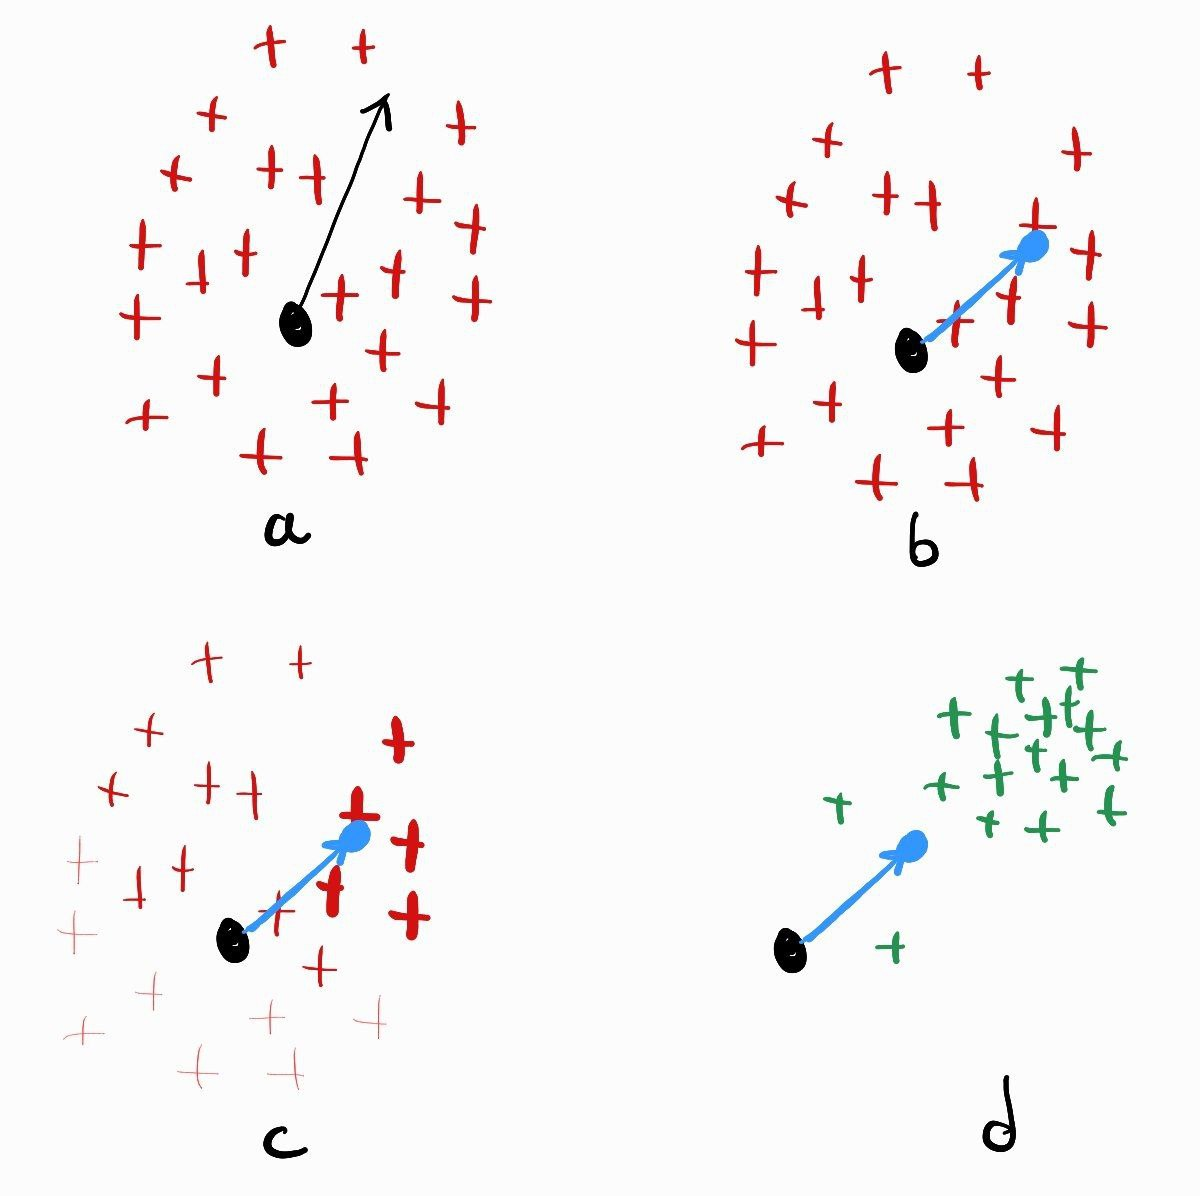
\includegraphics[width=0.4\textwidth]{Figures/pf.jpg}
    \caption{Representation of the model update.}
    \label{img:pf}
\end{figure}
\begin{itemize}
    \item[a.] At the beginning we have no idea what kind of behavior the object will have, it might be the black arrow, but we don't know, so we draw a set of samples in pretty much every direction and these samples will have the same weight at the very beginning.
    \item[b.] We observe a movement (blue arrow) and we take a measurement to know what are the particles that better approximate the object movement.
    \item[c.] Some of them are close, some are useless, we assign a weight to each particle based on the goodness of the approximation.
    \item[d.] Now instead of drawing new particles like in step $a)$ we draw more points in a certain direction, this will lead us to be more accurate, taking into account non-linear and non-gaussian behaviors but still keeping in the set of points some "outliers" in case the object decides to move in a different direction.
\end{itemize}


\begin{figure}[H]
    \centering
    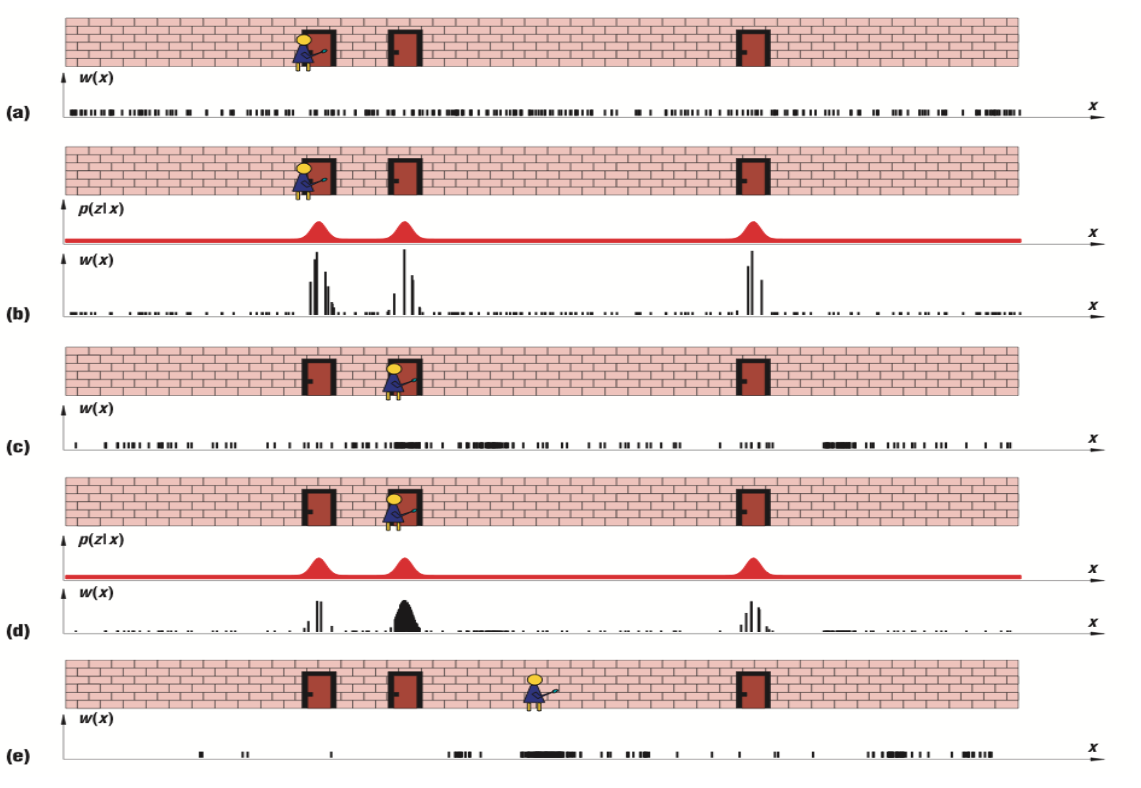
\includegraphics[width=0.9\textwidth]{Figures/pftoy.png}
    \caption{The PF solution to the toy problem we have previously seen for the Bayesian Tracking. Just as before we are provided with a door sensing device that will start ringing as we approach a door.}
    \label{img:pftoy}
\end{figure}

\begin{itemize}
    \item [(a)] At the beginning we select a certain distribution of the point which to us are potential solutions to the problem, but we have no idea where the guy can be. Any sample could potentially be a solution.
    \item [(b)] By the time the device rings it means we are close to one among the 3 doors. What happens is that instate of creating a continuous distribution, we assign a higher priority to the samples that are close to the doors, graphically we are increasing the bars of the points in proximity to the doors, and we assign less weight to the samples outside the range of the doors.
    \item [(c)] Given that we have assigned higher probability to these points, in the next step we draw more samples in the areas of higher probability, but before doing that, we need to propagate the information over time. As a result, we will have high density areas shifted from the peaks computed at step $(b)$ according to our model. The fact that we still have some sparse samples in the areas of low probability makes the algorithm more robust, as we would be able to "catch" the person in case he decided to move in a different direction compared to our prediction, in case this happened the redrawing of the samples would be done accordingly.
    \item [(d)] At a certain point he approaches the second door. Now we have again evidence that the guy is at one of the three locations, as a consequence we increase the probabilities of the samples in proximity of the doors. 
    \item [(e)] In this step we redraw the particles giving higher priority to the locations where we collected some evidence and we propagate according to the model.
\end{itemize}